\section{Implémentation de l'algorithme de correction d'erreur de phase}
\label{sec:choix_pga}

Pour l'implémentation de la correction d'erreur de phase, l'algorithme \textit{Phase Gradient Autofocus} (PGA) a été retenu. Cet algorithme est particulièrement robuste car il ne repose pas sur un modèle polynomial de l'erreur, permettant ainsi de corriger des distorsions de phase de fréquences élevées. Le détail de sa résolution est présenté ci-après.

L'objectif du PGA est d'estimer et de compenser le terme d'erreur de phase $\xi(x)$. La phase totale d'un signal reçu est cependant composite ; il est donc nécessaire d'isoler les termes d'intérêt en éliminant les composantes dites « parasites ». 

Dans la suite, nous distinguerons le \textbf{plan image} (données focalisées en pixels) du \textbf{plan signal} (données brutes après compression en distance, mais avant compression azimutale complète).

On définit l'expression de la phase du signal d'un pixel dans le plan image par :
\begin{equation}
\label{eq:phase}
    \Phi(x, y) \approx \frac{4 \pi}{\lambda} \left( R(x, y) + \xi(x) + \varphi(x, y) \right) 
\end{equation}
Où : 
\begin{itemize}
    \item $R(x, y)$ est la distance géométrique entre le capteur et la cible.
    \item $\xi(x)$ est l'erreur de phase induite par les défauts de trajectoire (que l'on cherche à estimer). 
    \item $\varphi(x, y)$ est la réponse de phase intrinsèque du diffuseur à la position $(x, y)$. 
\end{itemize}

En développant la distance $R(x, y) = \sqrt{R(y)^2 + (vt - x_0)^2}$ (où $v$ est la vitesse du porteur et $x_0$ la position de la cible) par une approximation paraxiale ($R(y) \gg x$), on obtient :
\begin{equation}
    \Phi(x, y) \approx \frac{4 \pi}{\lambda} \left( R(y) + \frac{(x - x_0)^2}{2R(y)} + \xi(x) + \varphi(x, y) \right)
\end{equation}

En considérant que le terme en $\frac{x^2}{2R(y)}$ est compensé lors de la formation de l'image, l'expression devient :
\begin{equation}
    \Phi(x, y) \approx \frac{4 \pi}{\lambda} \left( \underbrace{R(y) + \frac{x_0^2}{2R(y)} + \varphi(x, y)}_{\text{Termes constants}} - \frac{x \cdot x_0}{R(y)} + \xi(x) \right) 
\end{equation}

On observe un ensemble de termes constants sur l'axe azimutal pour une case de distance (\textit{range bin}) donnée. Pour les éliminer, l'algorithme estime le gradient de la phase. Toutefois, le terme $-\frac{x \cdot x_0}{R(y)}$, dépendant de l'azimut, subsisterait après dérivation (dépendance Doppler liée à l'excentricité de la cible).

Pour annuler ce terme, on réalise une étape de \textit{circular shifting} : pour chaque ligne (range bin), on identifie le diffuseur le plus brillant (\textit{dominant scatterer}) et on effectue une translation circulaire pour le centrer au milieu de l'image. Cela ramène $x_0$ à $0$, éliminant ainsi la rampe de phase linéaire. \cite{303752}

\begin{figure}[htbp]
    \centering
    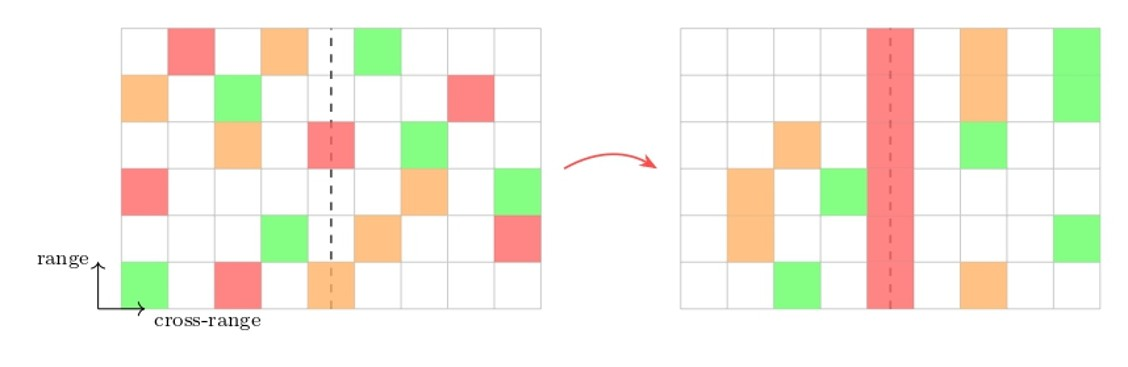
\includegraphics[width=0.7\linewidth]{src/rapport_complet/img/circ_shift.jpg}
    \caption{Principe du décalage circulaire (\textit{circular shifting}) pour le centrage des diffuseurs.}
    \label{fig:circshift}
\end{figure}

Ensuite, un fenêtrage est appliqué sur l'axe azimutal pour augmenter le SNR. Le signal fenêtré $s_c$ s'écrit :
\begin{equation}
    s_c(x - x_0, y) = \Pi_W(x) \cdot A(x - x_0, y) e^{-j \Phi(x - x_0, y)}
\end{equation}
Où $\Pi_W(x)$ est une fonction porte de largeur $W$. Cette largeur est réduite de manière itérative : plus l'image gagne en focalisation, plus la fenêtre est resserrée pour isoler le lobe principal du diffuseur.

Le passage dans le domaine fréquentiel azimutal permet alors d'isoler l'erreur de phase :
\begin{equation}
    s_c(x-x_0, y) \xrightarrow{\mathcal{F}_{az}} S_c(\eta, u) e^{-j2\pi x_0 u}
\end{equation}

L'estimation du gradient de la phase $\dot{\Phi}$ est réalisée par un estimateur de maximum de vraisemblance sur l'ensemble des $N$ \textit{range bins} \cite{303752} :
\begin{equation}
    \hat{\dot{\Phi}}(u) = \frac{\sum_{\eta=1}^{N} \Im\{S_c^*(\eta, u) \cdot \dot{S}_c(\eta, u)\}}{\sum_{\eta=1}^{N} |S_c(\eta, u)|^2} 
\end{equation}

Le résultat est ensuite intégré pour obtenir l'estimée de l'erreur $\hat{\xi}$, puis appliqué en correction. Le processus itère jusqu'à ce que la variation de l'erreur de phase soit inférieure à un seuil prédéfini. La structure globale est résumée en Figure \ref{fig:pga_custom}.
\begin{figure}[htbp]
    \centering
    \begin{tikzpicture}[node distance=1.3cm, font=\small, >=stealth, thick]
        % --- COLONNE 1 (Traitement Image) ---
        \node (start) [draw, rounded corners, fill=gray!10, text width=2.5cm, align=center] {Image SAR initiale};
        \node (shift) [draw, below of=start, fill=blue!15, text width=2.5cm, align=center, yshift=-0.5cm] {Décalage circulaire};
        \node (fft) [draw, below of=shift, fill=blue!15, text width=2.5cm, align=center, yshift=-0.5cm] {FFT Azimut};
        \node (ifft) [draw, below of=fft, yshift=-3.5cm, fill=blue!5, text width=2.5cm, align=center] {IFFT Azimut};

        % --- COLONNE 2 (Estimation et Correction) ---
        \node (est) [draw, right of=fft, xshift=3.5cm, fill=cyan!20, text width=3cm, align=center] {Estimation du gradient};
        \node (corr) [draw, below of=est, yshift=-0.5cm, fill=cyan!20, text width=3cm, align=center] {Correction de phase};
        \node (dec) [draw, diamond, aspect=2, below of=corr, yshift=-1.5cm, fill=orange!20, text width=2cm, align=center] {Stable ?};

        % --- COLONNE 3 (Sortie) ---
        \node (final) [draw, right of=dec, xshift=3.5cm, fill=green!20, text width=2.5cm, align=center] {Image Focalisée};

        % --- FLÈCHES ---
        \draw [->] (start) -- (shift);
        \draw [->] (shift) -- (fft);
        \draw [->] (fft) -- (est);
        \draw [->] (est) -- (corr);
        \draw [->] (corr) -- (dec);
        
        % Boucle de retour vers IFFT
        \draw [->] (dec.west) -- node[above, pos=0.5] {NON} ++(-1.5,0) |- (ifft.east);
        % Le fameux retour coudé de IFFT vers Shift
        % On sort par le nord, on monte un peu, on part à gauche, et on redescend vers l'ouest de shift
        \draw [dashed, ->] (ifft.north) -- ++(0,0.5) -- ++(-2,0) |- (shift.west);
        
        % Sortie finale
        \draw [->] (dec.east) -- node[pos=0.4, above] {OUI} (final.west);
    \end{tikzpicture}
    \caption{Fonctionnement de l'algorithme PGA}
    \label{fig:pga_custom}
\end{figure}
\FloatBarrier
Afin de valider l'implémentation et l'intégration de l'algorithme dans notre chaîne de traitement, une erreur de phase sinusoïdale est injectée dans l'historique de phase de l'image (obtenu par un passage dans le domaine spectral à partir de l'image finale). La figure \ref{fig:preuve-fig} présente l'image initiale, puis l'image dégradée après injection de l'erreur. On observe que l'impact de cette perturbation est significatif, générant des fantômes (duplications du point brillant) le long de l'axe azimutal.

La dernière image démontre l'efficacité de l'algorithme PGA, qui parvient à supprimer ces répliques tout en préservant la largeur du lobe principal et la position de la cible. Bien qu'un léger étalement de l'énergie soit perceptible en azimut, les niveaux de remontée du bruit restent inférieurs à ceux des premiers lobes secondaires d'un sinus cardinal (-13 dB). Ce résultat est jugé satisfaisant, validant ainsi la capacité de l'algorithme à restaurer la qualité image malgré des erreurs de phase cycliques. 
\begin{figure}
    \centering
    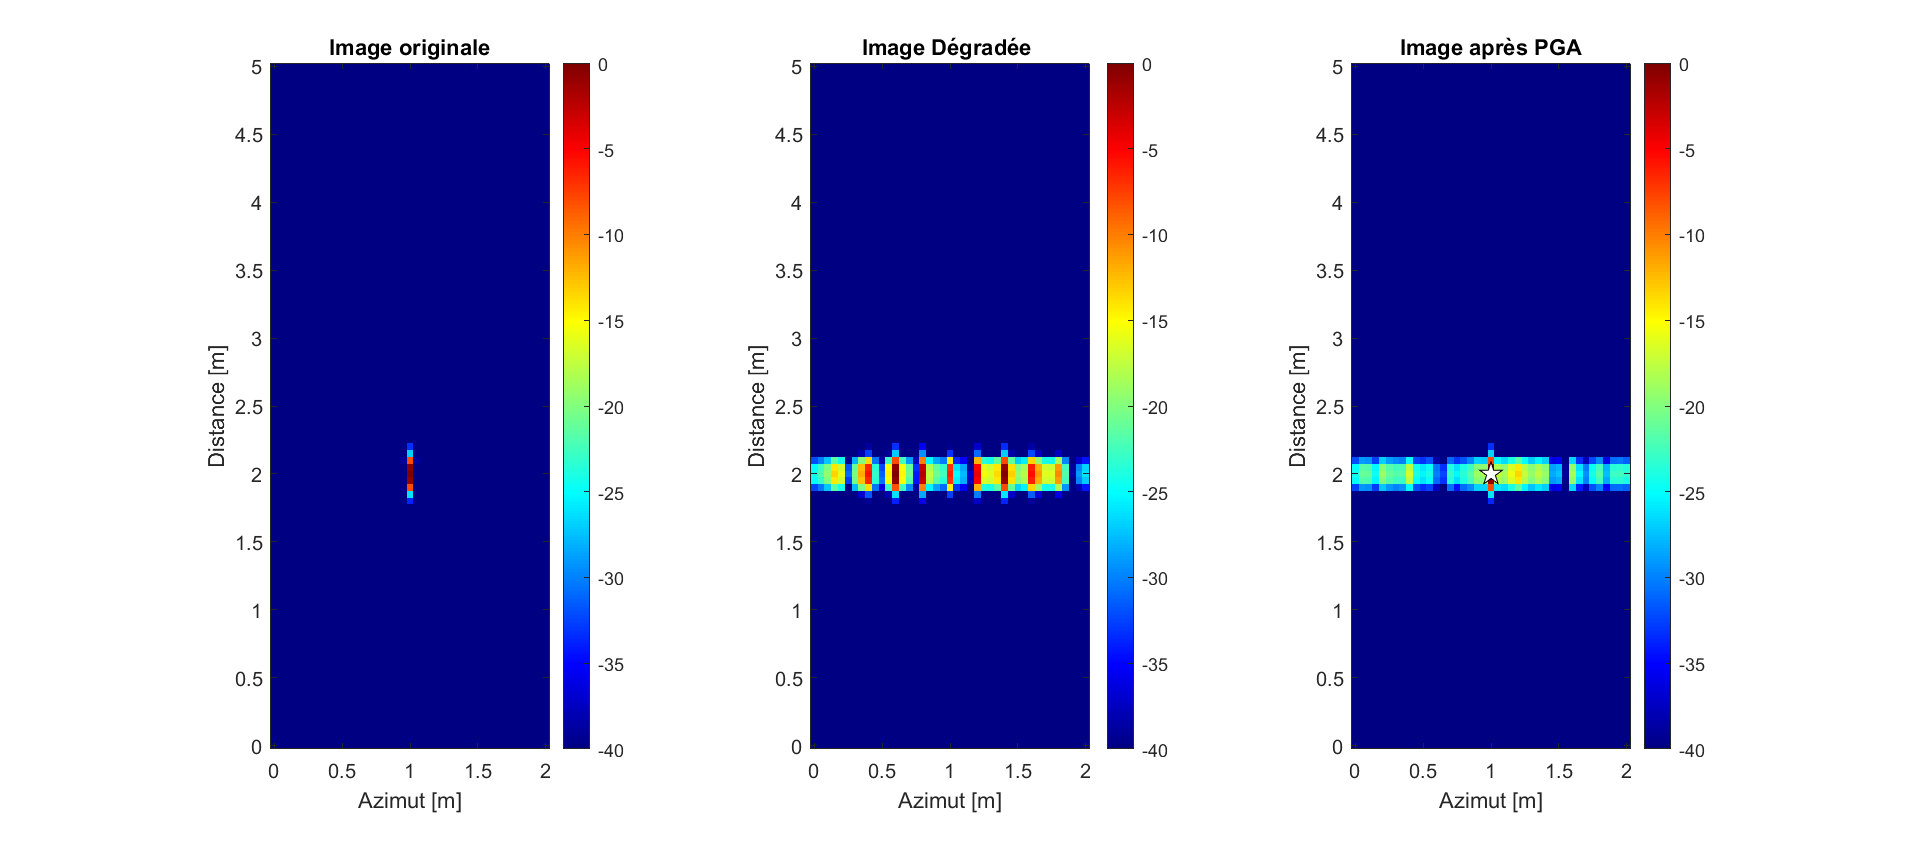
\includegraphics[width=0.7\linewidth]{src/rapport_complet/img/preuve_image_autofocus.png}
    \caption{Correctifs de PGA sur une image dégradée par une erreur sinusoïdale}
    \label{fig:preuve-fig}
\end{figure}
La figure \ref{fig:preuve-track} expose la superposition entre l'erreur de phase injectée et l'erreur estimée par l'algorithme. Cette comparaison témoigne de la fidélité de l'estimation, bien que l'on observe un léger effet de bord sur les derniers indices temporels, inhérent aux limites de fenêtre de l'estimateur. Toutefois, la quantification de l'erreur d'estimation résiduelle n'est pas l'objectif premier; la validation de l'algorithme repose ici sur une métrique de qualité image, à savoir la préservation de la largeur du lobe principal de la réponse impulsionnelle, garantissant le maintien de la résolution théorique. 
\begin{figure}
    \centering
    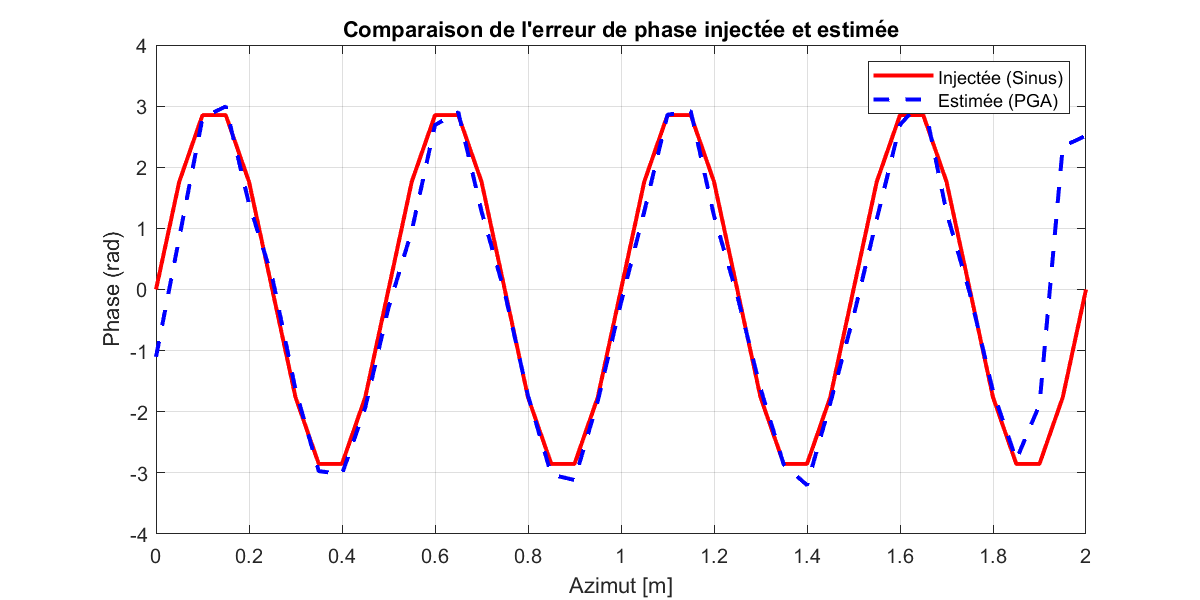
\includegraphics[width=0.7\linewidth]{src/rapport_complet/img/preuve_tracking_autofocus.png}
    \caption{Erreur de phase estimée et réelle}
    \label{fig:preuve-track}
\end{figure}
\FloatBarrier
Enfin, à mesure que les itérations progressent, l'erreur de phase résiduelle est censée diminuer, l'algorithme affinant l'estimation à chaque étape. Pour vérifier la convergence et le bon fonctionnement du traitement, on utilise la métrique RMS (Root Mean Square) de la phase estimée $\Phi(u)$, définie par :\begin{equation}\phi_{RMS} = \sqrt{\frac{1}{N} \sum_{u=1}^{N} \Phi(u)^2}\end{equation}On constate sur la figure \ref{fig:preuve-RMS} une décroissance monotone du RMS en fonction du rang de l'itération, ce qui confirme la convergence de l'algorithme PGA. Cette visualisation constitue également un indicateur de performance permettant de valider la cohérence des paramètres de l'estimateur (tels que la taille de la fenêtre de filtrage) vis-à-vis de la complexité de la scène observée.
\begin{figure}
    \centering
    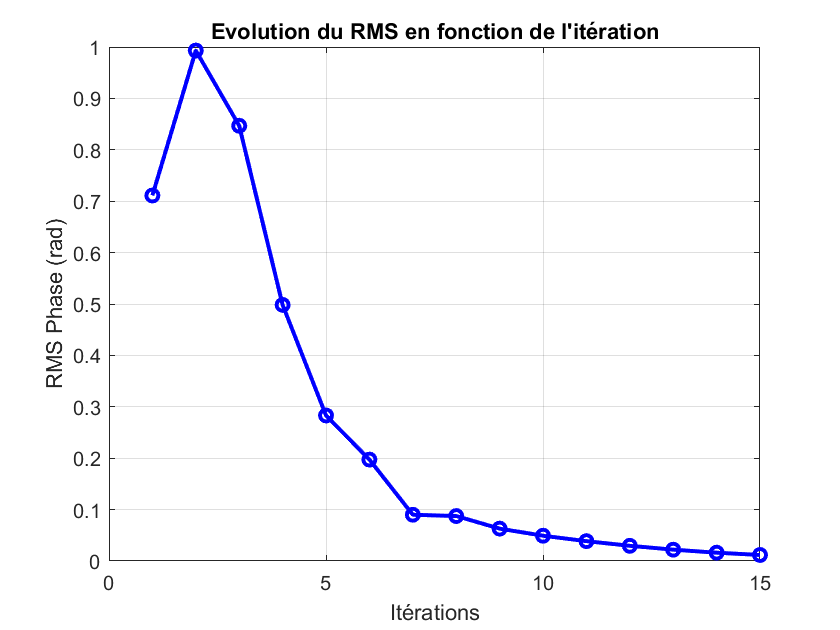
\includegraphics[width=0.7\linewidth]{src/rapport_complet/img/preuve_convergence_RMS.png}
    \caption{Evolution du RMS en fonction de l'itération}
    \label{fig:preuve-RMS}
\end{figure}

